%--------------------------------------------------
\section{Modelo-Lógico del sistema}
\begin{figure}[htbp!]
		\centering
			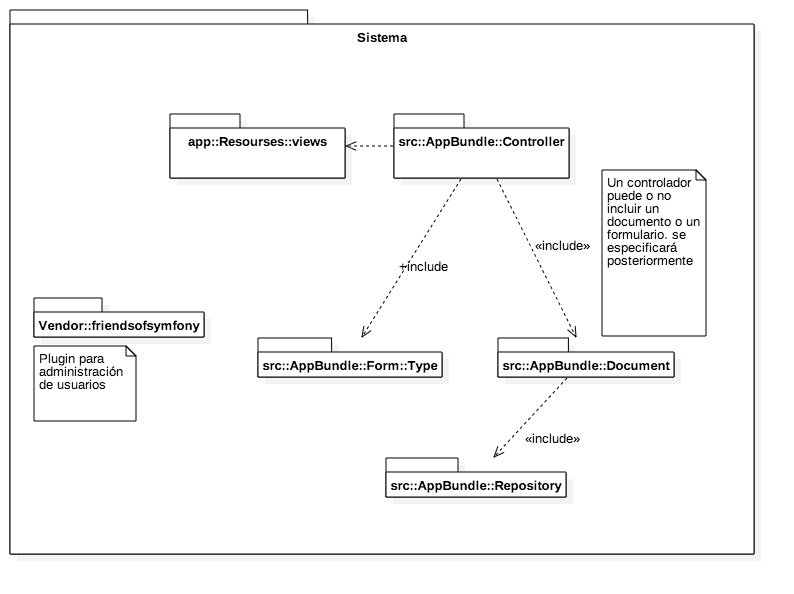
\includegraphics[width=1\textwidth]{images/logico31}
		\caption{Estructura general del sistema}
	\end{figure}

\begin{figure}[htbp!]
		\centering
			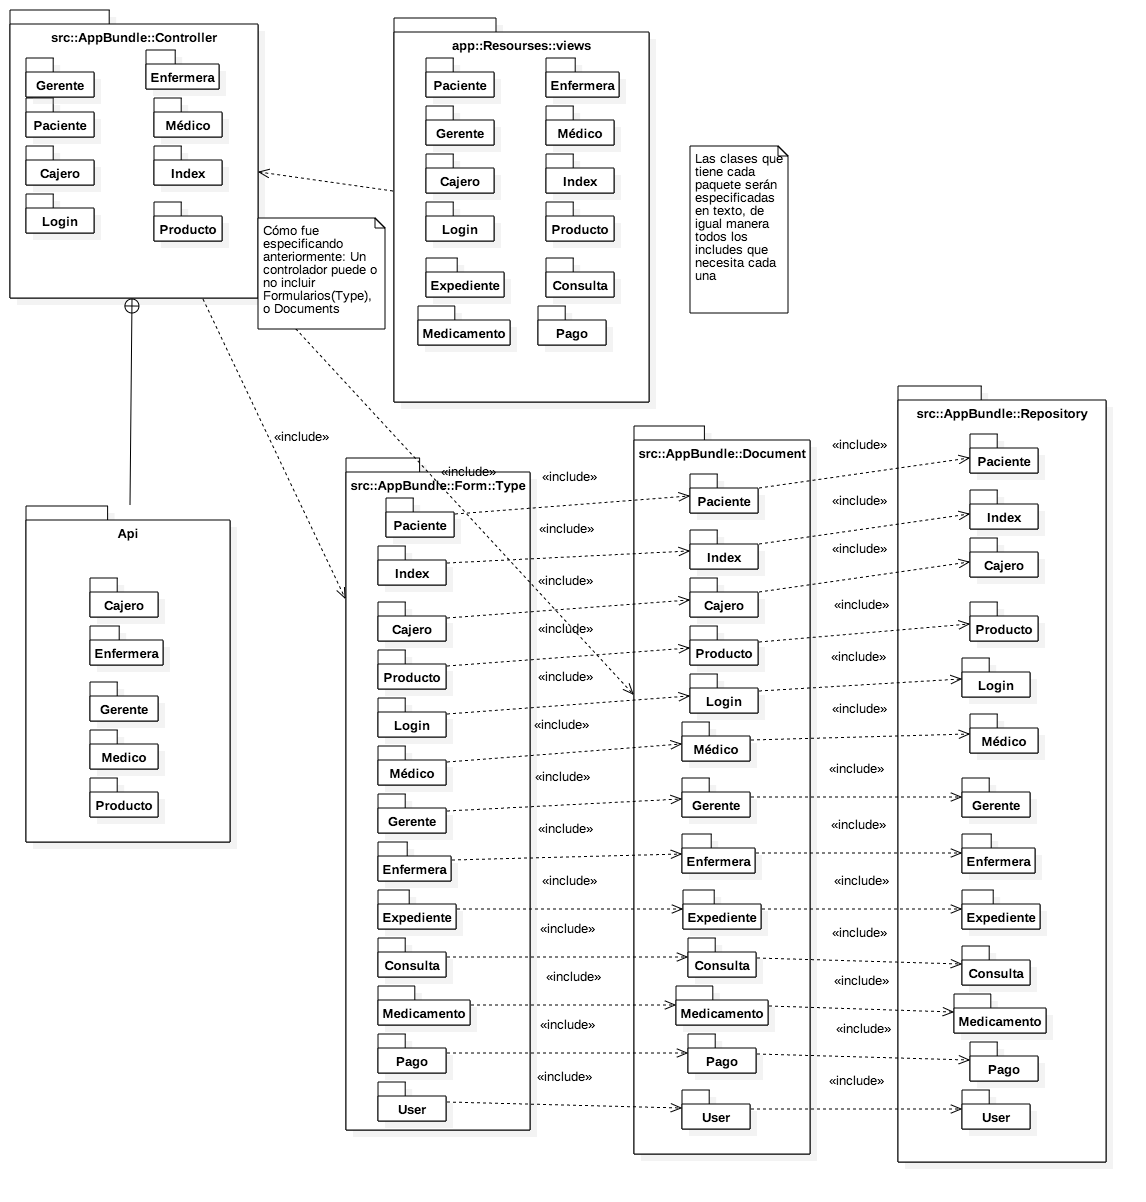
\includegraphics[width=1\textwidth]{images/logico32}
		\caption{Estructura Más especifica del sistema}
	\end{figure}
	
	\begin{figure}[htbp!]
		\centering
			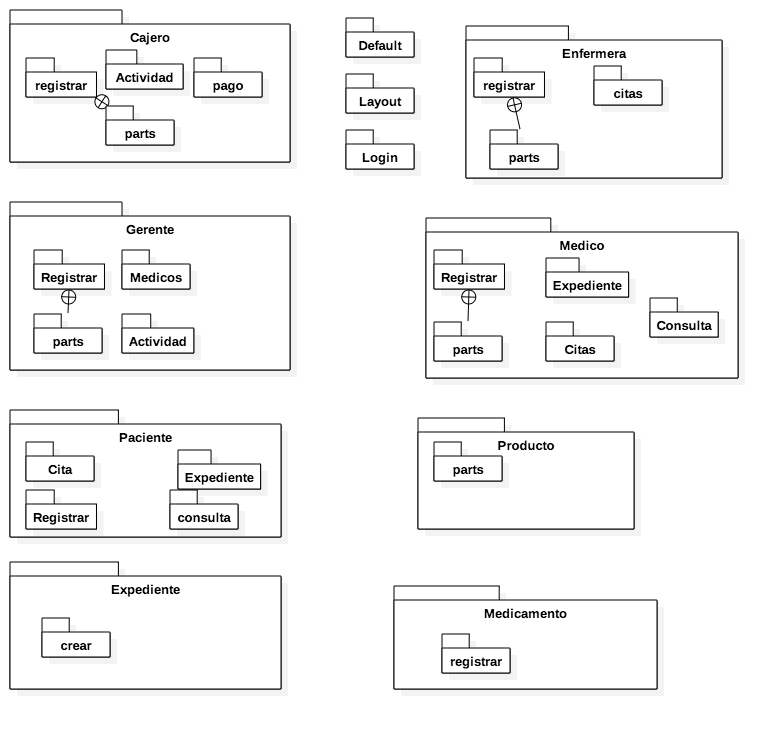
\includegraphics[width=1\textwidth]{images/logico33}
		\caption{Estructura de las vistas}
	\end{figure}
	\newpage
	\section{app::Resourses::views}
		\subsection{Cajero}
		\begin{itemize}
			\item Regjstrar
			\begin{itemize}
				\item parts
				\begin{itemize}
					\item cajeroTabla.html.twig
				\end{itemize}
				\item registrarCajero.html.twig
			\end{itemize}
			\item Inventario
			\begin{itemize}
				\item modificarInventario.html.twig
				\item consultarInventario.html.twig
			\end{itemize}
			\item Pagos
			\begin{itemize}
				\item pagoFarmacia.html.twig
				\item pagoCita.html.twig
			\end{itemize}
		\end{itemize}
		\subsection{Enfernera}
		\begin{itemize}
		\item Registrar
		\begin{itemize}
		\item registrarEnfermera.html.twig
		\item registrarPaciente.html.twig
		\item parts
			\begin{itemize}
				\item enfermeraTabla.html.twig
			\end{itemize}
		\end{itemize}
		\item citas 
			\begin{itemize}
				\item agendarCita.html.twig
				\item consultarCita.html.twig
				\item cancerlarCita.html.twig
			\end{itemize}
		\end{itemize}
		\subsection{Gerente}
		\begin{itemize}
			\item registrar
			\begin{itemize}
				\item parts 
				\begin{itemize}
				\item gerenteTabla.html.twig
				\end{itemize}
				\item registrarPaciente.html.twig
			\end{itemize}
			\item medicos 
			\begin{itemize}
			\item modifIcarHorarioMedico.html.twig
			\item registrarMedico.html.twig
			\item consultarMedicos.html.twig
			\end{itemize}
			\item actividad
			\begin{itemize}
				\item consultarCitasRealizadas.html.twig
				\item consultarVentasRealizadas.html.twig
			\end{itemize}
		\end{itemize}
		\subsection{Medico}
		\begin{itemize}
			\item registrar
			\begin{itemize}
			\item registrarMedico.html.twig
			\item parts
			\begin{itemize}
				\item medicoTabla.html.twig
			\end{itemize}
			\end{itemize}
			\item Expediente 
			\begin{itemize}
				\item crearExpediente.html.twig
				\item consultarExpediente.html.twig
			\end{itemize}
			\item citas
			\begin{itemize}
				\item consultarCitas.html.twig
				\item cancelarCitas.html.twig
			\end{itemize}
			\item consulta
			\begin{itemize}
				\item crearTratamiento.html.twig				
			\end{itemize}
		\end{itemize}
		\subsection{Paciente}
		\begin{itemize}
			\item cita
			\begin{itemize}
				\item agendarCita.html.twig
				\item cancelarCita.html.twig
			\end{itemize}
			\item expediente
			\begin{itemize}
				\item consultarExpediente.html.twig
			\end{itemize}
			\item registrar
			\begin{itemize}
			\item registrarPaciente.html.twig
			\end{itemize}
			
		\end{itemize}
		\subsection{Producto}	
			\begin{itemize}
			\item parts
			\begin{itemize}
				\item productosTabla.html.twig
			\end{itemize}
			\item registrarProducto.html.twig
			\end{itemize}

		\subsection{default}
		\begin{itemize}
			\item index.html.twig
		\end{itemize}
		\subsection{Login}
		\begin{itemize}
			\item login.html.twig
		\end{itemize}
		\subsection{Layout}
		\begin{itemize}
			\item menuLeft.html.twig
			\item menuTop.html.twig
		\end{itemize}
	\section{src::AppBundle::Controller}
	\subsection{Gerente}
	\begin{itemize}
		\item GerenteController.php
	\end{itemize}
	\subsection{Enfermera}
	\begin{itemize}
		\item EnfermeraController.php
	\end{itemize}
	\subsection{Paciente}
	\begin{itemize}
		\item PacienteController.php
	\end{itemize}
	\subsection{Medico}
	\begin{itemize}
		\item MedicoController.php
	\end{itemize}
	\subsection{Cajero}
	\begin{itemize}
		\item CajeroController.php
	\end{itemize}
	\subsection{Index}
	\begin{itemize}
		\item IndexController.php
	\end{itemize}
	\subsection{Login}
	\begin{itemize}
		\item LoginController.php
	\end{itemize}
	\subsection{Producto}
	\begin{itemize}
		\item ProductoController.php
	\end{itemize}
	\section{src::AppBundle::Controller::Api}
		\subsection{Cajero}
		\begin{itemize}
		\item CajeroController.php
		\end{itemize}
		\subsection{Enfermera}
		\begin{itemize}
		\item EnfermeraController.php
		\end{itemize}
		\subsection{Gerente}
		\begin{itemize}
		\item GerenteController.php
		\end{itemize}
		\subsection{Medico}
		\begin{itemize}
		\item MedicoController.php
		\end{itemize}
		\subsection{Producto}
		\begin{itemize}
		\item ProductoController.php
		\end{itemize}
	\section{src::AppBundle::Form::Type}
		\subsection{Paciente}
		\begin{itemize}
		\item CitaType.php
		\item PacienteType.php
		\end{itemize}
		\subsection{Index}
		\subsection{Cajero}
		\begin{itemize}
		\item CajeroRegistrationType.php
		\item CajeroType.php
		\end{itemize}
		\subsection{Producto}
		\begin{itemize}
		\item ProductoType.php
		\end{itemize}
		\subsection{Login}
		\subsection{Medico}
		\begin{itemize}
		\item MedicoRegistrationType.php
		\item MedicoType.php
		\end{itemize}
		
		\subsection{Gerente}
		\begin{itemize}
		\item GerenteRegistrationType.php
		\item GerenteType.php
		\end{itemize}
		
		\subsection{Enfermera}
		\begin{itemize}
		\item EnfermeraRegistrationType.php
		\item EnfermeraType.php
		\end{itemize}
		
		\subsection{Expediente}
		\subsection{Consulta}
		\subsection{Medicamento}
		\subsection{Pago}
		\subsection{User}
		\begin{itemize}
		\item RegistrationType.php
		\end{itemize}
	\newpage	
	\section{src::AppBundle::Document}
	
	\subsection{Paciente}
		\subsection{Cajero}
		\begin{itemize}
			\item Cajero.php
		\end{itemize}				
		
		\subsection{Producto}
		\begin{itemize}
			\item Producto.php
		\end{itemize}				
		
		\subsection{Medico}
		\begin{itemize}
			\item Medico.php
		\end{itemize}				
		
		\subsection{Gerente}
		\begin{itemize}
			\item Gerente.php
		\end{itemize}				
		
		\subsection{Enfermera}
		\begin{itemize}
			\item Enfermera.php
		\end{itemize}				
		
		\subsection{Expediente}
		\begin{itemize}
			\item Alergia.php
			\item AntecedenteFamiliar.php
			\item AntecedentePersonal.php
			\item Anticonceptivo.php
			\item Cirugia.php
			\item Embarazo.php
			\item Enfermedad.php
			\item Expediente.php
			\item Mastografía.php
			\item Papanicolaou.php
		\end{itemize}				
		
		\subsection{Consulta}
		\begin{itemize}
			\item Consulta.php
			\item Tratamiento.php
			\item TratamientoMedicamento.php
			\item TratamientoRecomendacion.php
		\end{itemize}
		\subsection{Medicamento}
		\begin{itemize}
			\item Activo.php
			\item Medicamento.php
		\end{itemize}
		\subsection{Pago}
		\begin{itemize}
			\item Pago.php
		\end{itemize}
		\subsection{User}
		\begin{itemize}
			\item User.php
		\end{itemize}
		
\section{src::AppBundle::Repository}
	
	\subsection{Paciente}
		\subsection{Cajero}
		\begin{itemize}
			\item CajeroRepository.php
		\end{itemize}
		\subsection{Producto}
		\begin{itemize}
			\item ProductoRepository.php
		\end{itemize}
		\subsection{Medico}
		\begin{itemize}
			\item MedicoRepository.php
		\end{itemize}
		\subsection{Gerente}
		\begin{itemize}
			\item GerenteRepository.php
		\end{itemize}
		\subsection{Enfermera}
		\begin{itemize}
			\item EnfermeraRepository.php
		\end{itemize}
		\subsection{Expediente}
		\begin{itemize}
			\item algo
		\end{itemize}
		\subsection{Consulta}
		
		\subsection{Medicamento}
		\begin{itemize}
		\item MedicamentoRepository.php
		\end{itemize}
		\subsection{Pago}
		\begin{itemize}
			\item PagoRepository.php
		\end{itemize}
		\subsection{User}
		\begin{itemize}
			\item UserRepository.php
		\end{itemize}%--------------------------------------------------


